%%%% imav.tex
% This is the tex-file for the IMAV 2014 conference
% for questions / remarks / bugs regarding the files, please contact info@imavs.org
% You can use this style for your conference, as long as you refer to the IMAV 2014
% in a comment similar to this one.
% Of course, the IMAV 2014 is not liable for any aspects of its use.

\documentclass{article}
% The style file
\usepackage{imav}
% Use the postscript times font!
\usepackage{times}
\usepackage{graphicx}
% \usepackage{algorithmic}
\usepackage{wasysym}
\usepackage{hyperref}
\usepackage{svg}
\usepackage{algorithm}
\usepackage{algpseudocode}
% \usepackage{algcompatible}
\usepackage{pifont}
\usepackage{wrapfig}
\usepackage[utf8]{inputenc}
\usepackage[T1]{fontenc}
% \usepackage[demo]{graphicx}
\usepackage{caption}
\usepackage{subcaption}
\usepackage{siunitx}
\usepackage{multirow}
\usepackage{amsmath}
\usepackage{array}
\usepackage{animate}

\usepackage{booktabs}
%%%%%% Add comment commands here %%%%%%%%%%%%%
\definecolor{YB}{RGB}{0,150,255}
\newcommand{\YB}[1]{\textcolor{YB}{YB: #1}}
\newcommand{\KVDB}[1]{\textcolor{green}{KVDB: #1}}
\newcommand{\TODO}[1]{\textcolor{red}{TODO: #1}}
\newcommand{\note}[1]{\textcolor{blue}{Note: #1}}
\newcommand{\red}[1]{\textcolor{red}{#1}}

\def\thickhline{\noalign{\hrule height.8pt}}
%%%%%%%%%%%%%%%%%%%%%%%%%%%%%%%%%%%%%%%%%%%%%%


\pagenumbering{none}
%\numberwithin{algorithm}{chapter}
%\usepackage{algorithmicx}
% the following package is optional:
%\usepackage{latexsym}

\title{Reinforcement Learning for a Neuromorphic Controller for UAV}
\author{K. Van den Berghe\\ \textit{Technische Universiteit van Delft, 1 Kluyverweg, Delft}\vspace{-0.5cm}}

% \renewenvironment{abstract}
%  {\small
%   \begin{center}
%   \bfseries \abstractname\vspace{-.5em}\vspace{0pt}
%   \end{center}
%   \list{}{
%     \setlength{\leftmargin}{0cm}%
%     \setlength{\rightmargin}{\leftmargin}%
%   }%
%   \item\relax}
%  {\endlist}

\begin{document}
% \pagenumbering{arabic}
\maketitle

\begin{abstract}
 This report presents a study on the application of reinforcement learning to train spiking neural networks (SNNs) for controlling a micro aerial vehicle (MAV) during landing. SNNs, inspired by biological neurons, offer potential for low-power and event-based computation but pose significant training challenges. The methodology combines supervised pre-training and two spiking reinforcement learning algorithms—Deep Q-Networks (DQN) and Advantage Actor-Critic (A2C)—to enable effective training. The controller, consisting of layers of leaky integrate-and-fire (LIF) neurons, was pre-trained to extract velocity information from sonar measurements. The model was then refined using reinforcement learning to enhance its landing performance.

Experimental evaluations were conducted in multiple environments, including a simplified simulator, the PaparazziUAV simulator, and a real drone, demonstrating the generalization capability of the trained SNN. Results indicate that while the SNN successfully managed landing tasks, it exhibited slow training processes and issues with dead and saturated neurons, highlighting areas for improvement. Future work aims to integrate recurrent replay buffers and explore stochastic neuron models to enhance training efficiency and address neuron inactivity.
\end{abstract}

\section{Introduction} \label{section:introduction}
Spiking neural networks (SNNs) are a bio-inspired model of neural computation that use spikes to represent and process information. While SNNs have the potential for low-power event-based computation, training them effectively remains a challenge. This report presents using a reinforcement learning approach for training SNNs to control a micro aerial vehicle (MAV) during landing.

A key difference between SNNs and traditional artificial neural networks is that SNNs operate on spike sequences over time rather than activation values. This necessitates adaptations to common deep learning algorithms for training SNNs. The presented pipeline first uses supervised pre-training to help the SNN learn meaningful representations for the control task. It then fine-tunes the network using two spiking reinforcement learning algorithms: a spiking version of Deep Q-Networks (DQN) and Advantage Actor-Critic (A2C).

The spiking DQN algorithm is modified from the standard DQN to learn from interaction sequences instead of single state-transitions. A2C is also adapted for the spiking domain, again avoiding the shuffling and batching of the interactions. The trained SNN controller is then evaluated in a physics simulator and on the real system. The results provide insights into effective reinforcement learning methods for training SNNs to solve real-world control problems.

\section{Related work} \label{section:lit_review} 
Existing research in the field of neuromorphic Reinforcement Learning (RL) has mainly applied one algorithm; deep Q learning (DQN). The deep Q algorithm is a well established algorithm, introduced by DeepMind. The original publication demonstrated the performance of this algorithm on multiple Atari games, displaying its versatility~\cite{mnih2013playing}. It is a simple and elegant algorithm, based on tabular Q-learning, that uses an artificial neural network as policy. One component, important in the performance of this algorithm, is the experience replay~\cite{fedus_revisiting_2020}. During the training phase, experience from previous environment interactions is used together with the most recent experience to avoid bias in the training data and improve training characteristics. The spiking variant of this algorithm has been demonstrated in earlier work. DSQN has been applied on the Atari environments and on the Airsim environment and outperform several ANN based solutions~\cite{DSQN_Atari, DQN_Atari_human-level_2022, DSQN_AirSim}. One drawback of current implementations is that temporal information is not exploited. They use rate encoding techniques, running several forward passes per input, decreasing efficiency and undermining the temporal learning capabilities of SNN. The implementations used in this report make use of sequences for training where a linear layer is used for encoding sensor data to the spiking domain, closely resembling a population encoding mechanism. 

Neuromorphic control has been applied on Micro Aerial Vehicles (MAV) \cite{Stroobants2022DesignProcessors, Stroobants2022NeuromorphicQuadrotors, Vitale2021Event-drivenChip, Paredes-Valles2023FullyFlight}, aiming to exploit the promises of energy efficiency and latency from neuromorphic algorithms. This stream of work spans manual tuning to supervised training methods for developping low level controllers, to full end to end control. A neuromorphic PID controller was manually tuned and demonstrated for onboard attitude control \cite{Stroobants2022DesignProcessors}. Next to control, an SNN has been successfully used for attitude estimation in highly dynamic environments, using IMU data \cite{Stroobants2022NeuromorphicQuadrotors}. End-to-end control was later demonstrated on the Intel Loihi chip \cite{Davies2018Loihi:Learning}. The network used optical flow, trained in an unsupervised setting, for vertical control of an MAV \cite{Paredes-Valles2023FullyFlight}.

% The previous work on SNN based RL algorithms span a wide array of different environments, tasks and training methods. Early research already harnessed bio-inspired training algorithms such as spike-timing-dependent plasticity (STDP)~\cite{STDP_survey}. STDP is commonly described as: \textit{cells that fire together, wire together}. It is a concept derived from neuroscience, that assumes that neurons that often spike simultaneously, probably represent the same information. R.V. Florian\cite{florian_reinforcement_2005} proposed an algorithm based on deep Q learning, modulating the STDP with the global reward signal, for a bio-inspired problem. The agent controls a worm that solves a localization problem based on gradient descent, receiving a positive reward if it comes closer to the source, while receiving a negative reward when moving to a region with a lower concentration. Further work shows that using reward modulated spike-timing-dependent plasticity (R-STDP) or temporal difference spike-timing-dependent plasticity (TD-STDP) allows networks to train more complex tasks such as the CartPole~\cite{liu_spiking_2023}, a task where the model has to balance a stick on a cart, by only applying a force to the cart~\cite{CartPole}. However, the model showed slow convergence and noisy, imperfect results. Another method inspired by neuroscience is eProp. This method showed to approach the performance of backpropagation through time for recurrent SNN~\cite{eProp_pong}.
\\
% Methods that more closely resemble the training of non-spiking networks, include shadow training and surrogate gradient training. In shadow training~\cite{ding2021optimal}. We train an ANN and convert it to an SNN based agent. This approach, however, has shown to produce worse performing models compared to the ANN based equivalent and to a DQN algorithm directly optimizing the SNN based agent (DSQN)\cite{ding_chen_deep_2022}. This is explained by the fact that the converted SNN will always be limited by the ANN from which it is converted, while the other two methods (DQN and DSQN) train directly from the environment. Surrogate gradient training~\cite{neftci2019surrogate} overcomes the non-differentiable of spikes by modelling the step function that presents the spiking behaviour of a neuron, with a differentiable surrogate function that approaches the step function the backward pass.


\section{Methods}
\label{section:methods}
Building on previous work on spiking implementations of DQN and A2C, SNN based controllers can be trained on custom environments. The task of the SNN consisted in landing an MAV as fast as possible, without exceeding a predefined landing velocity, using only sonar altitude readings. Due to the implicit recurrence of spiking neurons, it was hypothesized that SNN would be able to estimate velocity and land the vehicle without the need for explicitly recurrent layers. The engineering process for this training pipeline was meticulously designed and comprised several steps. Firstly, a lightweight simulator was constructed to replicate pertinent dynamics while providing rapid simulation for efficient training. To expedite the learning process, a pre-training task was devised. It was observed that without proper guidance, the network encountered difficulties in developing an internal representation of velocity, which is crucial for calculating the necessary thrust to guarantee safe landings. This pre-trained network then underwent further training using A2C and DQN algorithms. Ultimately, the controller was integrated into a simulation environment and subsequently deployed on a physical drone using PaparazziUAV, showcasing its real-world applicability.
 \subsection{Spiking Neural Network}
 The architecture used for the controller consists of 2 hidden layers, each with 32 leaky integrate-and-fire (LIF) neurons, connected with linear feedforward layers. The input, which is the altitude read by the sonar, is passed to the first layer without encoding. The output is discretized to 7 neurons, each corresponding to an acceleration command. A softmax function is applied to the membrane potentials, from which the action can be extracted. During training, the time constants and thresholds related to the neurons are trained together with the weights.
 
\subsection{Pretraining}
In the field of reinforcement learning (RL), spiking neural networks (SNNs) often face challenges due to their relatively slow training process. However, a simple yet effective solution to enhance their performance lies in incorporating a pretraining task focused on improving scene understanding. It was observed that SNNs trained directly with RL struggled to retrieve a velocity representation, which is crucial to land the MAV. However, when performing a supervised pretraining task, where the SNN learns velocity given sonar readings, the network significantly outperformed the networks only trained by RL, saving significant computational resources and speeding up the training process by an order of magnitude.

\subsection{Simulator}\label{simulator}
The training is conducted in a simple environment designed to increase training speed, featuring rudimentary dynamics. The real MAV is controlled using throttle inputs. However, in simulation, the model outputs a target acceleration with respect to the hover acceleration, which are passed through a low-pass filter. Acceleration commands are between $-1 \frac{m}{s^2}$ and $1 \frac{m}{s^2}$. The dynamics are then described by the following equations:
\begin{align}\label{eq:dynamics}
\Dot{h}t &= \Dot{h}{t-1} + \Ddot{h}t \cdot \Delta t \\
h_t &= h{t-1} + \Dot{h}_t \cdot \Delta t \
\end{align}
Where $h$ is the altitude, $\Dot{h}$ is the vertical velocity and $\Ddot{h}$ is the vertical acceleration after passing through the low-pass filter. \\

To enhance the controller's robustness, the starting altitude, and starting velocity are varied across episodes. The agent receives the altitude as its observation, requiring the network to learn a derivative of the altitude, a task unsolvable for conventional feedforward neural networks. 


\subsection{Reinforcement Learning}
With the pretrained network, the training process for the lander can begin. By employing a spiking version of the A2C algorithm \cite{A3C, A2CvsA3C} and utilizing the dynamics model described in \autoref{simulator}, a spiking neural network can be trained to solve the task. Alternatively, a spiking version of DQN \cite{mnih2013playing}, which replaces transitions in the replay buffer with sequences of transitions, was also used for training a model. However, this approach resulted in very noisy training and failed to generalize to a reliable lander.

Previous research on reinforcement learning for temporal information has demonstrated that actor-critic methods outperform the unstable value function methods \cite{HeessMemory-basedNetworks, Yang2021RecurrentControl, Ni2021RecurrentPOMDPs}. Our findings confirm this, as the actor-critic approach proved more effective than the value function methods, which struggled to maintain stability.

\subsection{Deployment on the Parrot Bebop 2}
After training on the basic simulator, the model is deployed in the PaparazziUAV framework \cite{brisset2006Paparazzi}, an open-source UAV autopilot platform that facilitates fast, iterative development, targeting the Parrot Bebop 2 MAV. When the algorithm is verified within the PaparazziUAV simulation framework, the controller can be deployed on the real Parrot Bebop 2 MAV.

\section{Results}\label{sec:results}
To thoroughly evaluate the landing algorithm's ability to generalize across various dynamics with differing levels of complexity, its performance was compared across three environments: second-order dynamics, the PaparazziUAV simulator, and a real MAV. Notably, the same model, without any additional tuning or training, was employed across all simulators.

Initially, the algorithm's performance was assessed using the simple simulator. As illustrated in \autoref{fig:basic performance}, when the MAV starts with a non-zero velocity, the network promptly responds by issuing positive thrust commands to reduce the downward velocity. As the MAV approaches the ground, the network progressively increases the thrust, further slowing the descent. This behavior demonstrates the network's capacity to modulate thrust based on proximity to the landing surface and its internal representation of velocity.

It's important to note that the reward structure during training was designed to avoid excessively slow landings. Specifically, the MAV was not rewarded further for achieving landing speeds slower than $0.3 \frac{m}{s}$, as such slow landings were impractical and inefficient. This reward mechanism ensured that the network aimed for a balance between safety and efficiency during the landing process, promoting practical landing speeds without compromising the algorithm's effectiveness.
\begin{figure}[h!]
    \centering
    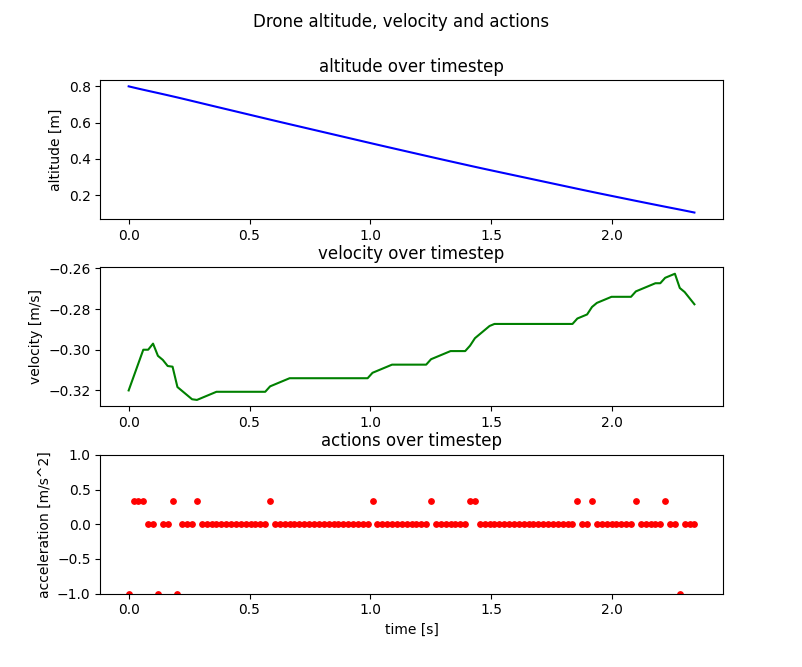
\includegraphics[width=.45\textwidth]{Figures/drone_landing_seed50_drone_snn_pos_06-05-02.png}
    \caption{Performance of an SNN based controller on the basic simulation model.}
    \label{fig:basic performance}
\end{figure}

To analyze whether the network exploits the velocity information rather than applying a fixed thrust, an experiment was run with a zero initial velocity. Now, the network is initially hesitant in commanding negative acceleration commands, slowing down the landing. When the network achieved approached landing, the network commanded more and more positive acceleration, slowing down the MAV upon landing as seen on \autoref{fig:Performance0vel}.

\begin{figure}[h!]
    \centering
    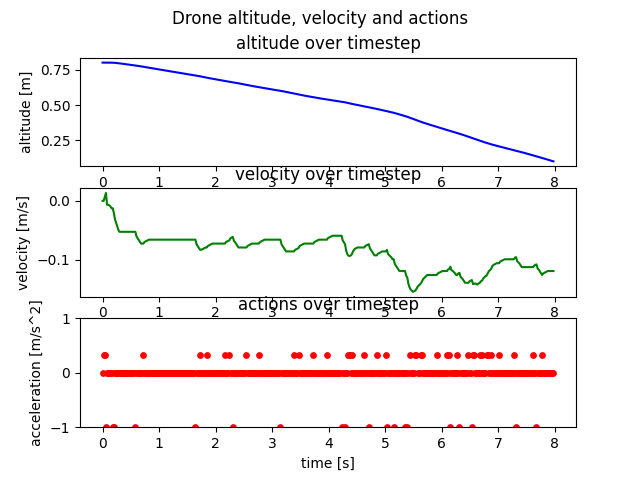
\includegraphics[width=.45\textwidth]{chapters/drone_landing_seed3_v00_drone_snn_pos_06-05-02.png}
    \caption{Performance of an SNN based controller on the basic simulation model, with a zero initial velocity.}
    \label{fig:Performance0vel}
\end{figure}

Next, the same network was deployed in the PaparazziUAV simulator environment. In this setup, the network's acceleration commands were mapped to throttle settings for the Parrot Bebop 2 MAV. To facilitate this, the model was converted into C code, which was then wrapped in a module compatible with PaparazziUAV. This C code is wrapped in a module, which can be used by a PaparazziUAV airframe. The airframe defines the characteristics of the MAV, the sensors that will be used and the controllers that control the MAV. Then, a flight plan is set up, which defines the trajectory to be followed. The flight plan consists of a take-off, a short standby period, and the landing with the SNN based controller.
Due to the coarse discretization of the controller, which outputs only seven distinct commands, the MAV's ability to finely adjust the thrust settings was limited. To address this, the range of thrust settings was constrained between $10\%$ and $70\%$, ensuring that the controller could effectively manage the MAV's thrust within these bounds.

Finally, the network was deployed on the real MAV. It was found that slight instabilities occurred which were not present in simulation. While this could partially be caused by the coarseness of the output actions, but are most likely caused by imperfect tuning of the underlying stabilization controllers, which were provided by the PaparazziUAV framework. On \autoref{fig:real_drone}, the path of the MAV is provided, for the interested reader, a video has been provided as well\footnote{\url{https://youtu.be/16wEXy7pPSM}}.
\begin{figure}
    \centering
    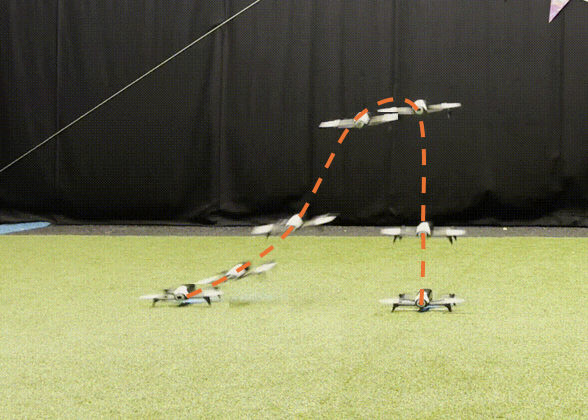
\includegraphics[width=.45\textwidth]{Figures/drone_landing/Drone_Landing_Burst.png}
    \caption{The controller deployed on the real MAV can successfully land}
    \label{fig:real_drone}
\end{figure}



\section{Conclusion and Future Work}
This report describes the development of a pipeline that enables training spiking neural network based controllers for landing MAVs.
While the described method successfully lands an MAV, it is not without its flaws. The spiking neural network (SNN) required pre-training tasks to extract velocity information from sequences of sonar measurements. Only after this pre-training could the reinforcement learning (RL) pipeline commence. However, training SNNs with RL proved to be significantly slower than training comparable artificial neural networks (ANNs). The trained SNN exhibited numerous dead and saturated neurons—neurons that either never spike or always spike, respectively—indicative of inefficient training. This inefficiency stems from the sparse gradients within the network and the weak learning signal, which is a characteristic challenge in RL. Additionally, the discrete set of output actions was suboptimal for control tasks. 

For future work, there are several avenues I would like to explore. First, I plan to investigate the application of findings from the original R2D2 publication \cite{kapturowski2018recurrent_r2d2}, particularly those related to recurrent replay buffers, to an off-policy, policy gradient reinforcement learning algorithm. This could potentially eliminate the need for pre-training. Next, I aim to combine this approach with an asymmetric actor-critic network \cite{pinto2017asymmetric}. In this setup, the actor, an SNN deployed on the real MAV, would receive the inputs observed by the MAV, while the critic, an ANN, would process all states available in the simulation and, optionally, explicitly receive a state history at every forward pass. This combination could enable faster and more stable training.

Another interesting direction is to explore stochastic neuron models that become more deterministic as training progresses. This approach could encourage greater network activity and address the issue of dead and saturated neurons. Additionally, balancing exploration and exploitation during training is crucial in reinforcement learning. This balance could be inherently encoded in the SNN agent, simplifying the training pipeline and potentially leading to more efficient training.

\input{chapters/06-Recommendations}


% BIBLIOGRAPHY:
% use {unsrt}:
\bibliographystyle{unsrt}
\bibliography{imav_bibliography}

% Supplementary materials
% \newpage

\section{Supplementary material}
Using NeuroBench to analyze the performance of the algorithms on the tasks allows us to return the histograms for all of the algorithms. These histograms show the results of all 1000 runs and show how consistently a model is able to perform its task.
\begin{figure}[h]
    \centering
    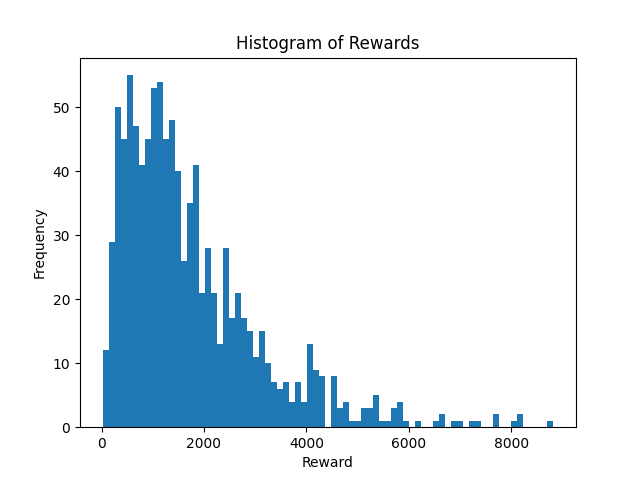
\includegraphics[width = .45\textwidth]{Figures/ANN_histogram1K.png}
    \caption{Histogram for the ANN with one hidden layer of size 246.}
    \label{fig:enter-label}
\end{figure}

\begin{figure}[h]
    \centering
    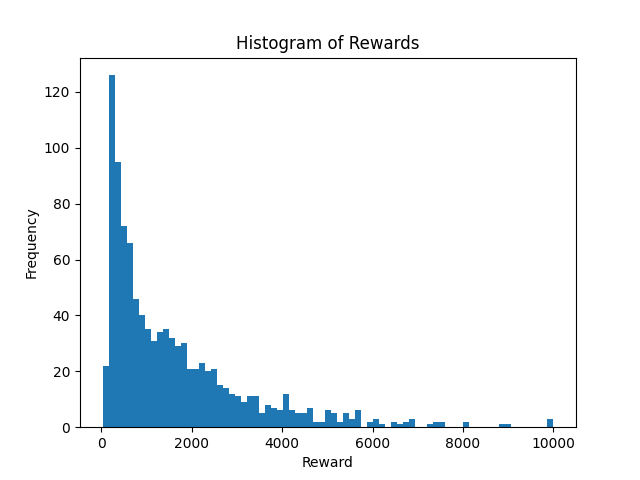
\includegraphics[width = .45\textwidth]{Figures/SNN_histogram1K_noLeak.png}
    \caption{Histogram for the SNN with one hidden layer of size 246, no leak.}
    \label{fig:enter-label}
\end{figure}

\begin{figure}[h]
    \centering
    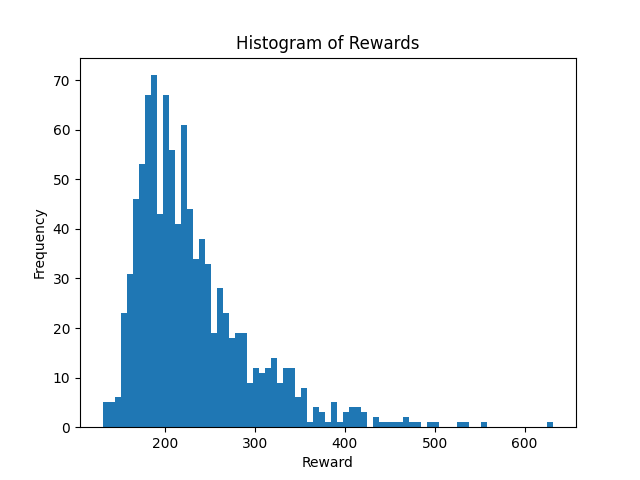
\includegraphics[width = .45\textwidth]{Figures/SNN_histogram1K_higher_leaks.png}
    \caption{Histogram for the SNN with one hidden layer of size 246, with $\beta=0.65$}
    \label{fig:enter-label}
\end{figure}


\end{document}

